\section{eo\-Bit\-Mutation$<$ Chrom $>$ Class Template Reference}
\label{classeo_bit_mutation}\index{eoBitMutation@{eoBitMutation}}
eo\-Bit\-Mutation --$>$ classical mutation  


{\tt \#include $<$ga/eo\-Bit\-Op.h$>$}

Inheritance diagram for eo\-Bit\-Mutation$<$ Chrom $>$::\begin{figure}[H]
\begin{center}
\leavevmode
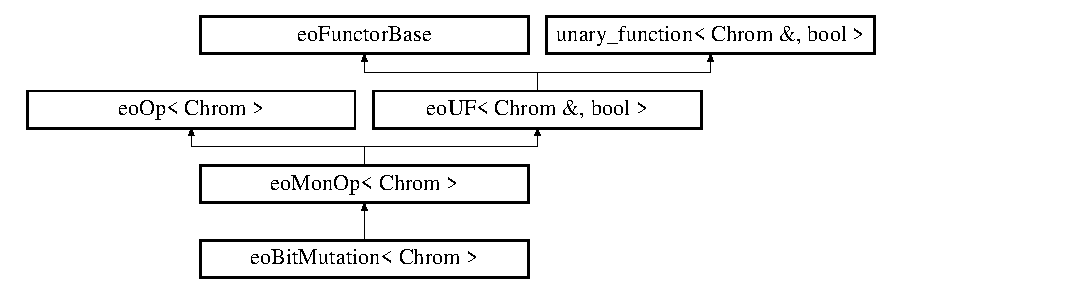
\includegraphics[height=3.50548cm]{classeo_bit_mutation}
\end{center}
\end{figure}
\subsection*{Public Member Functions}
\begin{CompactItemize}
\item 
{\bf eo\-Bit\-Mutation} (const double \&\_\-rate=0.01, bool \_\-normalize=false)
\begin{CompactList}\small\item\em (Default) Constructor. \item\end{CompactList}\item 
virtual std::string {\bf class\-Name} () const \label{classeo_bit_mutation_a1}

\begin{CompactList}\small\item\em The class name. \item\end{CompactList}\item 
bool {\bf operator()} (Chrom \&chrom)
\begin{CompactList}\small\item\em Mutate a chromosome. \item\end{CompactList}\end{CompactItemize}
\subsection*{Private Attributes}
\begin{CompactItemize}
\item 
double {\bf rate}\label{classeo_bit_mutation_r0}

\item 
bool {\bf normalize}\label{classeo_bit_mutation_r1}

\end{CompactItemize}


\subsection{Detailed Description}
\subsubsection*{template$<$class Chrom$>$ class eo\-Bit\-Mutation$<$ Chrom $>$}

eo\-Bit\-Mutation --$>$ classical mutation 



Definition at line 104 of file eo\-Bit\-Op.h.

\subsection{Constructor \& Destructor Documentation}
\index{eoBitMutation@{eo\-Bit\-Mutation}!eoBitMutation@{eoBitMutation}}
\index{eoBitMutation@{eoBitMutation}!eoBitMutation@{eo\-Bit\-Mutation}}
\subsubsection{\setlength{\rightskip}{0pt plus 5cm}template$<$class Chrom$>$ {\bf eo\-Bit\-Mutation}$<$ Chrom $>$::{\bf eo\-Bit\-Mutation} (const double \& {\em \_\-rate} = {\tt 0.01}, bool {\em \_\-normalize} = {\tt false})\hspace{0.3cm}{\tt  [inline]}}\label{classeo_bit_mutation_a0}


(Default) Constructor. 

\begin{Desc}
\item[Parameters:]
\begin{description}
\item[{\em \_\-rate}]Rate of mutation. \end{description}
\end{Desc}


Definition at line 111 of file eo\-Bit\-Op.h.

\subsection{Member Function Documentation}
\index{eoBitMutation@{eo\-Bit\-Mutation}!operator()@{operator()}}
\index{operator()@{operator()}!eoBitMutation@{eo\-Bit\-Mutation}}
\subsubsection{\setlength{\rightskip}{0pt plus 5cm}template$<$class Chrom$>$ bool {\bf eo\-Bit\-Mutation}$<$ Chrom $>$::operator() (Chrom \& {\em chrom})\hspace{0.3cm}{\tt  [inline, virtual]}}\label{classeo_bit_mutation_a2}


Mutate a chromosome. 

\begin{Desc}
\item[Parameters:]
\begin{description}
\item[{\em chrom}]The chromosome to be mutated. \end{description}
\end{Desc}


Implements {\bf eo\-UF$<$ Chrom \&, bool $>$} {\rm (p.\,\pageref{classeo_u_f_a1})}.

Definition at line 121 of file eo\-Bit\-Op.h.

The documentation for this class was generated from the following file:\begin{CompactItemize}
\item 
eo\-Bit\-Op.h\end{CompactItemize}
